\documentclass[CS5104-Notes.tex]{subfiles}
\begin{document}

\section{Deep learning}
In the basic equation for statistical prediction, we have
\begin{equation}
  \hat{Y} = f(X, \theta)
\end{equation}
which leads us to variations of linear functions with linear and logistic regression. There is a direct relation between the inputs and outputs but the simplicity of the model meant that it could only predict on linear data. More complex non-linear models were achieved by transforming the input data into new expanded feature spaces with an additional layer of processing
\begin{equation}
x \rightarrow h_{m}(x) \rightarrow y
\end{equation}
where $x$ is the original input data and $h_{m}(x)$ is the additional processing to transform the input space. This transformation can be done in multiple different ways for different models and techniques
\begin{itemize}
\item Basis expansions
\item Non-linear kernels
\item Hidden layers consisting of multiple neurons
\end{itemize}
We can see a pattern here of the models becoming ``deeper'' and requiring more processing as more complexity is needed. Moreover, feature extraction is often necessary and many steps of the feature extraction and feature mapping process were done by hand. The idea of \textbf{deep learning} is to learn all parts of the entire process from the data and be an end-to-end model.
\n
In general, deep learning refers to algorithms which learn from intermediate representations with more than one layer of intermediate representation, for example hierarchical Bayes networks or Markov random fields. However these days, deep learning often refers to \textbf{deep neural networks}.

\subsection{Deep neural network}
In essence, a deep neural network is simply a feedforward network with many hidden layers. The learning algorithm must decide how to use the layers to produce the desired output. Each layer in the deep neural network performs feature mapping, which can expand or reduce the feature space depending on both the weights and the number of neurons in each layer. A deep enough network can therefore represent arbitrarily complex functions.
\begin{figure}[H]
  \centering
  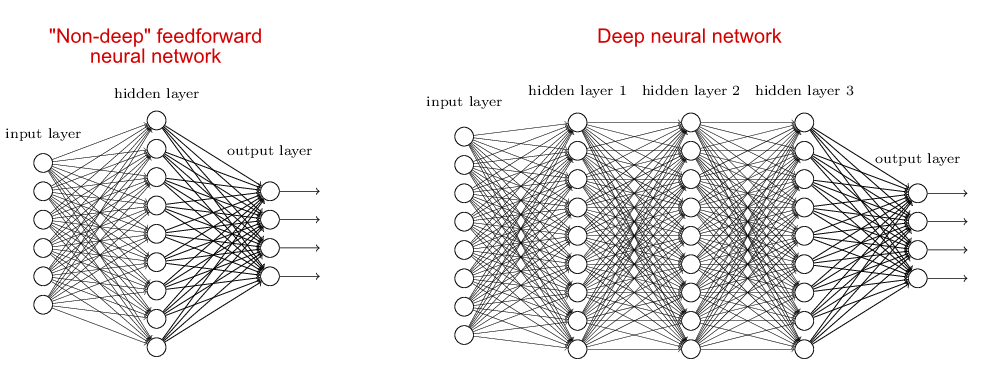
\includegraphics[width=1\textwidth, keepaspectratio]{imgs/deep-neural-network.png}
  \caption{A deep neural network simply has many hidden layers compared to a normal neural network.}
\end{figure}
\noindent
There are many problem that come with deep neural networks
\begin{itemize}
\item Computational complexity
\item Availability of data
\item Overfitting
\item Non-convex cost function
\item Vanishing gradient problem
\item Network topology (choosing the depth and width)
\end{itemize}

\subsubsection{Vanishing gradient problem}
Typically in neural networks, a sigmoid function
\begin{equation}
f(x) = \frac{1}{1 + e^{-x}}
\end{equation}
is used for classification, however an issue with these functions is the gradients become too small. The small gradient is propagated across the layers, which results in a very slow learning/training process.
\begin{figure}[H]
  \centering
  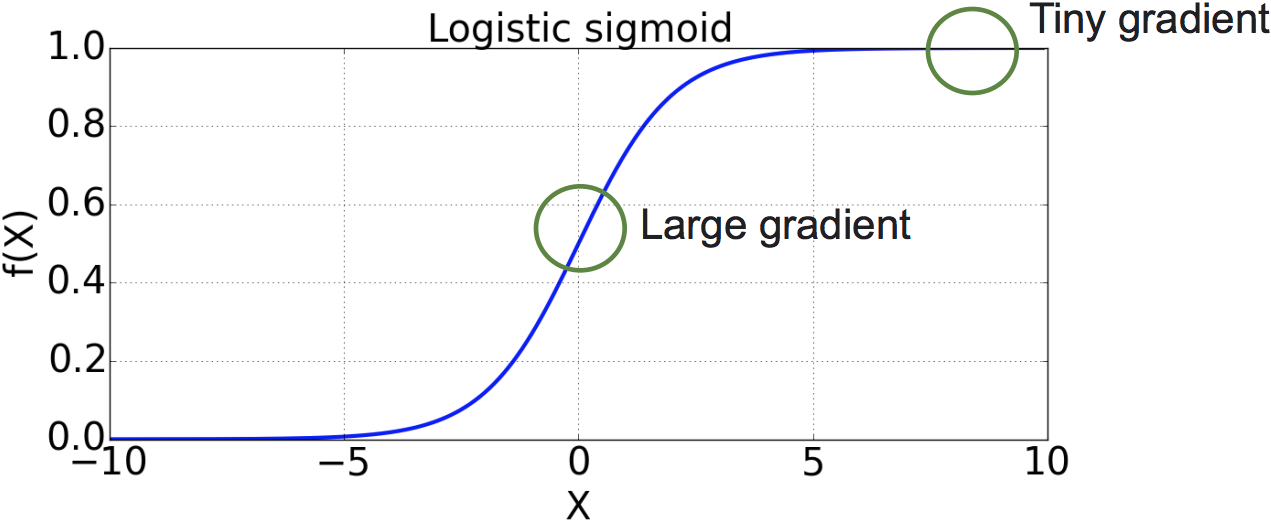
\includegraphics[width=0.8\textwidth, keepaspectratio]{imgs/vanishing-gradient-problem.png}
  \caption{Example of the small gradient on sigmoid-type functions.}
\end{figure}
\noindent
The issue is the simoid units saturate across most of the domain, saturating to a high value when $X$ is very positive, a low value when $X$ is very negative and only strongly sensitive in their input when $X$ is near 0. This makes learning difficult, which is why sigmoid units are not used often in feedforward networks. They can still work in gradient-descent based algorithms as the cost functions can undo the saturation of the sigmoid in the output layer.
\n
Instead \textbf{rectified units} can be used which lead to much faster learning. Rectified linear units used the activation function
\begin{equation}
\text{max}\{0, x\}
\end{equation}
The main difference with rectified units compared to linear or sigmoid units is that a rectified unit outputs zero across half of its domain. This makes the derivatives through a rectified unit remain large whenever the unit is active, making it more useful for learning.
\begin{figure}[H]
  \centering
  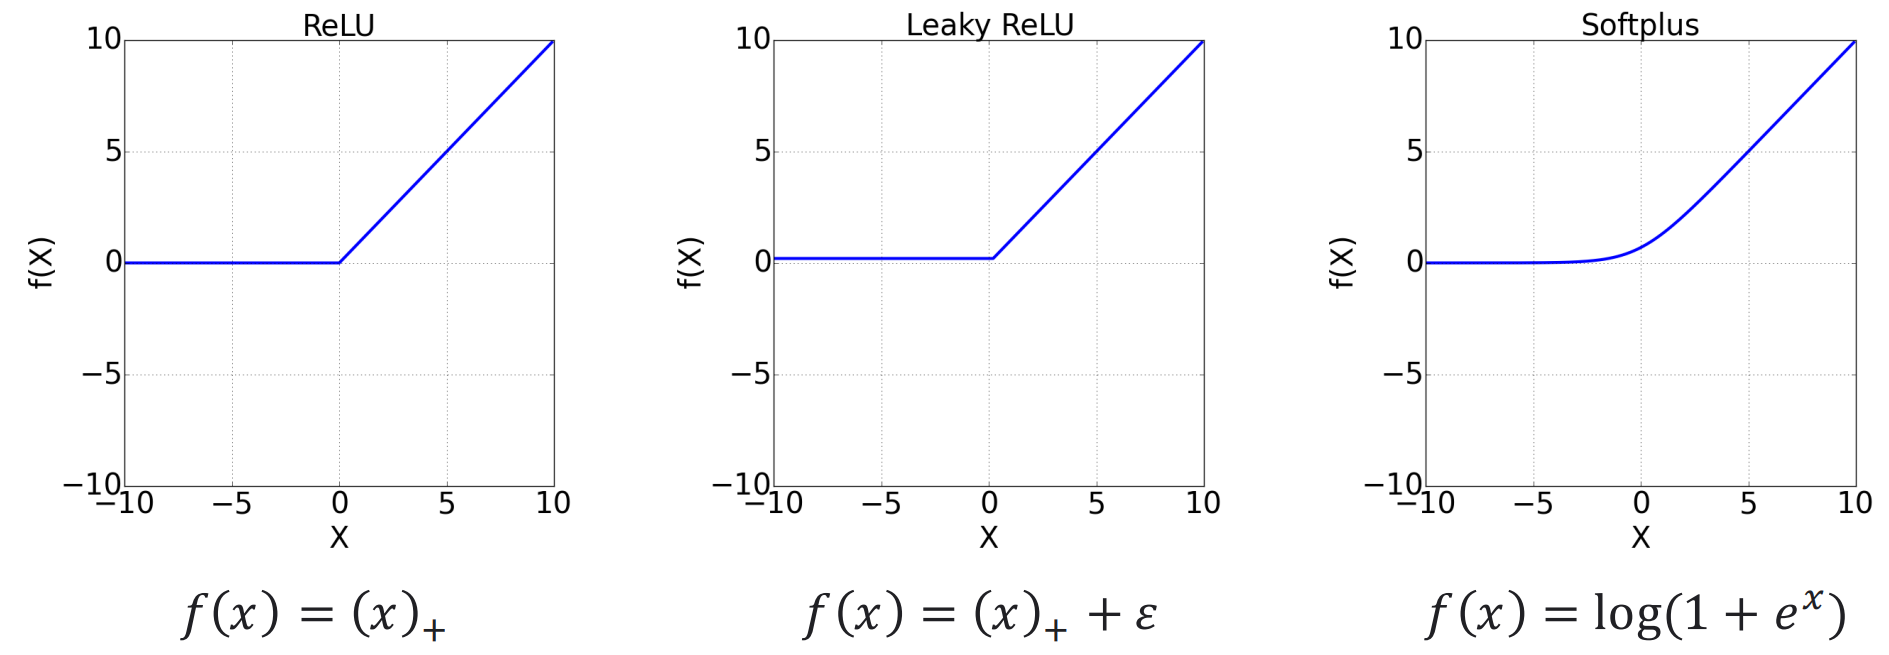
\includegraphics[width=1\textwidth, keepaspectratio]{imgs/rectified-units.png}
\end{figure}
\noindent
One drawback of rectified units is that they cannot learn via gradient-descent when their activation is zero. Furthermore, the linear units lead to large values, which often need to be re-normalised for each layer separately.

\subsection{Regularisation}
There are many forms of regularisation, which all attempt to decrease overfitting and allow predictive models to better generalise to unseen data. This is generally a trade-off of increasing the bias by only decreasing the variance by a small amount. Some forms of regularisation in deep neural networks resemble reguarlisation methods seen before, but there are also extensions to the basic concepts that apply particularly for neural networks.

\subsubsection{Norm penalities}
Many regularisation approaches are based on limiting the capacity of models by adding a parameter norm penalty $\Omega(\theta)$ to the objective function $J$
\begin{equation}
J(\theta) = L + \Omega(\theta)
\end{equation}
there $L$ is the loss function used. For example, the $l_{2}$ norm can be used as the norm penalty, which gives
\begin{equation}
J(\theta) = L + \frac{\lambda}{2}\sum_{i,j,l,i \neq 0}(\theta){i,j}^{(l)})^{2}
\end{equation}
Note the bias weights $\theta_{0,j}$ are left unregularised.

\subsubsection{Early stopping}
When training and adjusting weights with backpropagation, often the training error is calculated to ensure it continues to fall. However, if the model starts to overfit to the data, the training error can continue to fall even if the validation error begins to rise. This is especially common with complex models.
\begin{figure}[H]
  \centering
  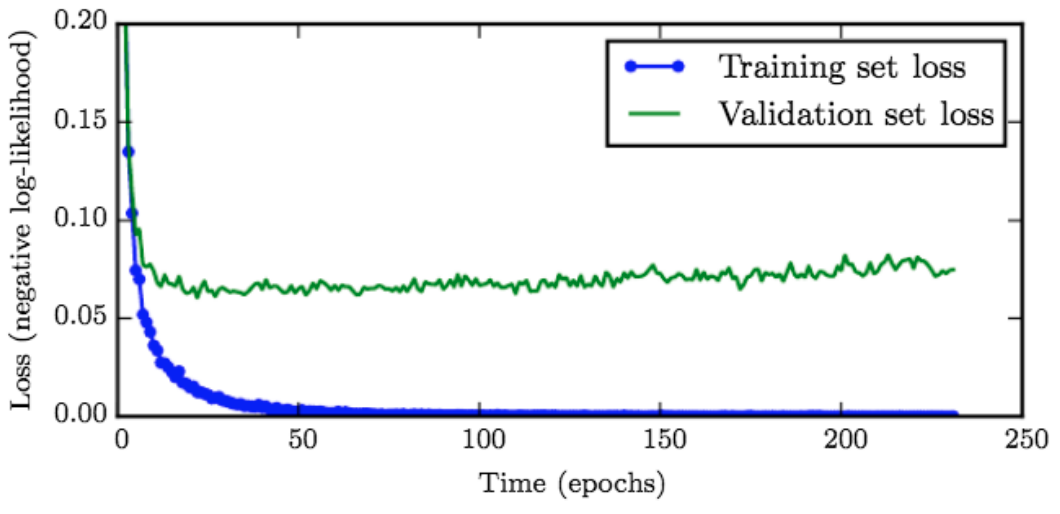
\includegraphics[width=0.6\textwidth, keepaspectratio]{imgs/early-stopping.png}
\end{figure}
\noindent
To prevent this, early stopping can be used to record good parameter values and stop if the validation error goes up when the training error goes down. 

\subsubsection{Dropout}
Dropout regularisation provides an inexpensive but powerful method of regularising a broad family of models. In simple terms, dropout can be thought of as practical bagging for many large neural networks. \textbf{Bagging} is the idea of training multiple models and choosing the best one based on the evaulation with test data. This is normally impractical because of the computational cost. Dropout is the approximation to training and evaluating a bag of exponentially many neural networks.
\n
In neural networks, particular units in the network can be effectively removed by multiplying its output value by zero. On each iteration
\begin{itemize}
\item Sample a different binary mask vector $\mu$ to apply to all input and hidden units in the network
\item Nodes where values of $\mu$ are zero are dropped
\item Only a subset of the data is trained
\item Sample again and repeat
\end{itemize}
Only a tiny fraction of the possible subnetworks are each trained for a single step, and the parameter sharing causes the remaining subnetworks to arrive at good settings of the parameters.
\begin{figure}[H]
  \centering
  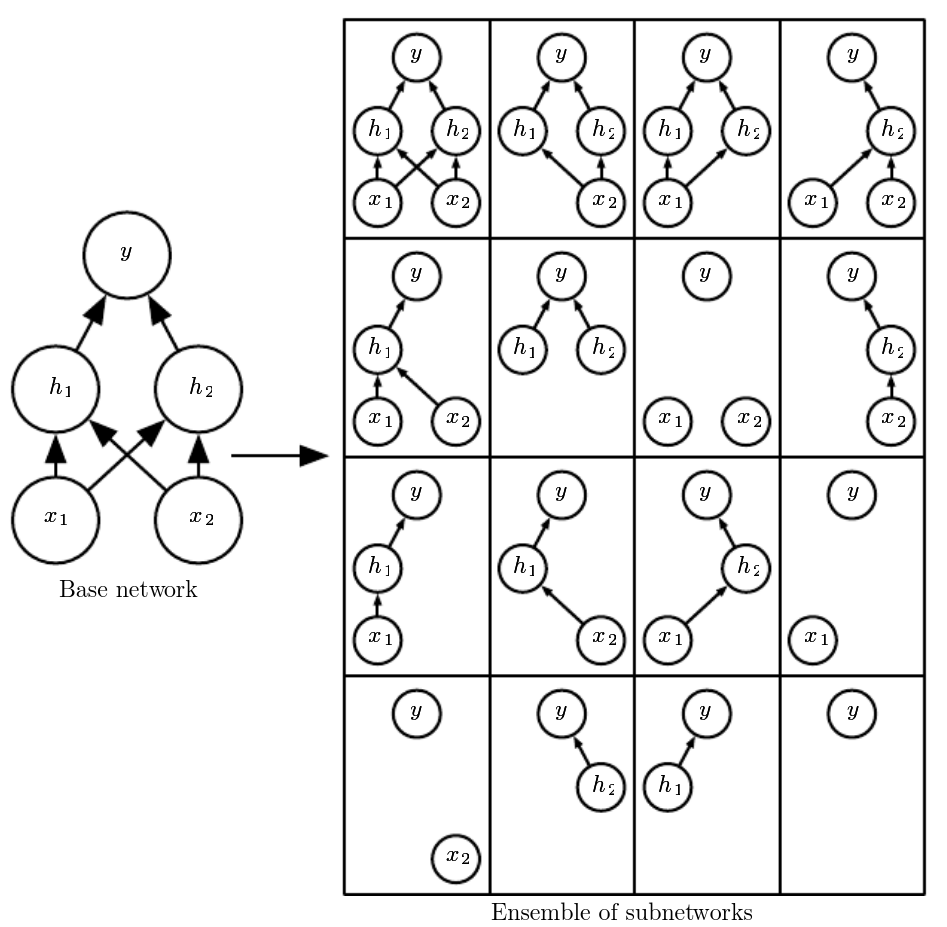
\includegraphics[width=0.6\textwidth, keepaspectratio]{imgs/dropout.png}
  \caption{The subnetworks are constructed by removing non-output units from an underlying base network.}
\end{figure}
\noindent
To create the subnetworks practically during forward propagation, the vector $\mu$ is randomly sampled with one entry for each input or hidden unit in the network. The entries of $\mu$ are binary (0 or 1) and are independent of each other. The probability of the entries being 1 is a hyperparameter that has to be set, it is typically 0.5 for hidden units and 0.8 for input units. Each unit in the network is then multiplied by the corresponding mask and forward propagated as normal. This is equivalent to selecting one of the sub-networks and running forward propagation through it.

\subsection{Batch optimisation}
As we typically wish to minimise the \textbf{mean} error in our model, we can average the error over all training samples at each iteration of the algorithm. This is known as \textbf{batch} gradient descent. Calculating the mean over the entire training set estimates the mean over all data, including the mean cost and mean gradient. In this approach, having more data leads to better estimates.

\subsubsection{Minibatch optimisation}
Gradients can be computed in batches of $n$ samples points at once, or rather $n$ epochs using $m$ minibatches in the same time. Such learning algorithms are typically called \textbf{stochastic} as a subset of the training set is randomly chosen to propagate the error and update parameters until convergence.
\n
The batch size is governed by a number of considerations, most notably:
\begin{itemize}
\item Amount of parallelism available
\item Amount of memory available
\item Batch size requirements (for example batches must be of size power of two)
\item Larger batches provide a more accurate estimate of the gradient, but with less than linear returns
\end{itemize}

\subsubsection{Stochastic gradient descent}
An example of a minibatch approach to gradient descent is the stochastic gradient descent. Instead of using the entire dataset, only a batch of datapoints are sampled. The mean cost and gradient for each parameter is calculated, which updates the parameters and direction of the gradient. This is repeated with new random samples until convergence.
\n
Furthermore, the learning rate \textit{decreases with time}. This is done because the sampling process introduces an error and the algorithm would never converge otherwise.

\subsubsection{Batch noramlisation}

\subsubsection{Parameter sharing}


\subsection{Concolutional neural networks}
\end{document}